\documentclass[12pt,compress,aspectratio=169]{beamer}
\usetheme{metropolis}
\setbeamersize{text margin left=.5cm,text margin right=.5cm}
\usepackage[lf]{carlito}
\usepackage{siunitx}
\usepackage{tikz}
\usepackage{mathpazo}
\usepackage{bm}
\usepackage{mathtools}
\usepackage[ISO]{diffcoeff}
\diffdef{}{ op-symbol=\mathsf{d} }
\usepackage{xcolor,colortbl}

\setmonofont{Ubuntu Mono}
\setlength{\parskip}{0pt}
\renewcommand{\baselinestretch}{1}

\sisetup{
  inter-unit-product=\cdot,
  per-mode=symbol
}

\tikzset{
  >=latex
}

%\newcommand{\iii}{\hat{\bm\imath}}
%\newcommand{\jjj}{\hat{\bm\jmath}}
%\newcommand{\kkk}{\hat{\bm k}}


\usetikzlibrary{decorations.pathmorphing,patterns}


\title{Class 3: Work and Energy}
\subtitle{Advanced Placement Physics C}
\author[TML]{Dr.\ Timothy Leung}
\institute{Olympiads School}
\date{Updated: Summer 2022}

\newcommand{\pic}[2]{
  \includegraphics[width=#1\textwidth]{#2}
}
\newcommand{\eq}[2]{
  \vspace{#1}{\Large
    \begin{displaymath}
      #2
    \end{displaymath}
  }
}
%\newcommand{\iii}{\ensuremath\hat{\bm{\imath}}}
%\newcommand{\jjj}{\ensuremath\hat{\bm{\jmath}}}
%\newcommand{\kkk}{\ensuremath\hat{\bm{k}}}
\newcommand{\iii}{\ensuremath\hat\imath}
\newcommand{\jjj}{\ensuremath\hat\jmath}
\newcommand{\kkk}{\ensuremath\hat k}



\begin{document}

\begin{frame}
  \maketitle
\end{frame}



\begin{frame}{Work and Energy}
  We start with some definition at are (unfortunately) not very useful:
  \begin{itemize}
    \item \textbf{Energy} is the ability to do work.
    \item \textbf{Work} is the mechanism in which energy is transformed.
  \end{itemize}
  Luckily, we can also use equations to define these concepts.
\end{frame}


\section{Work}

\begin{frame}{Work}
  \textbf{Mechanical work} $\dl W$ is done when a force $\vec F(x)$ displaces an
  object by $\dl\vec x$. If the force moves an object from  $\vec x_0$ to
  $\vec x_1$, the total work done by the force is defined as:

  \eq{-.1in}{
    \boxed{
      W=\int_{x_0}^{x_1}\vec F(\vec x)\cdot\dl\vec x
    }
  }

  \begin{itemize}
  \item Work is a scalar quantity
  \item No work done if the force is perpendicular to displacement, when
    $\vec F\cdot\dl\vec x=0$ (i.e.\ the force did not cause the displacement)
  \item No work done if no displacement ($\dl\vec x=\vec 0$)
  \item Work can be positive or negative depending on the dot product
  \end{itemize}
\end{frame}



\begin{frame}{In One Dimension}
  For motion confined to one dimension (which is common for AP Physics C), we
  can ignore the dot product:
  
  \eq{-.1in}{
    W=\int_{x_0}^{x_1} F(x)\dl x
  }

  (Direction still matters for $F$ and $x$, even in 1D, in that there is still
  a positive and negative direction.)
\end{frame}



\begin{frame}{Work by Constant Force}
  For a constant force, if the object moves along straight path, the integral
  simplifies to just the dot product of the two vectors:

  \eq{-.1in}{
    \boxed{
      W=\vec F\cdot\Delta\vec x
    }
  }

  In scalar form that is more familiar in Grades 11/12 Physics:

  \eq{-.1in}{
    \boxed{W=|\vec F||\Delta\vec x|\cos\theta}
  }

  where $\theta$ is the angle between the force and displacement vectors
\end{frame}



\begin{frame}{Definition of Work}
  \textbf{Work done by a force}
  \begin{itemize}
  \item The work done by \emph{one specific force}
  \item Example: A boy pushes a cart forward. The ``work done by the boy'' is
    the work done by the applied force.
  \end{itemize}

  \vspace{.15in}\textbf{Work done on an object}
  \begin{itemize}
  \item There may be more than one force acting on an object
  \item The \emph{sum} of all the work done on the object by each force
  \item The work done by the net force
  \item Also called the \textbf{net work} $W_\text{net}$
  \end{itemize}
\end{frame}



\section{Kinetic Energy \& Work-Energy Theorem}

\begin{frame}{Kinetic Energy}
  When a net force on an object (with constant mass) accelerates it, the
  resulting amount of work done on the object (net work $W_\text{net}$) is
  given by:

  \eq{-.1in}{
    W_\text{net}
<<<<<<< HEAD
    =\int_{x_0}^{x_1}F_\text{net}\dl x
=======
    =\int_{x_0}^{x_1}F_\text{net}(x)\dl x
>>>>>>> 2022-09-fall
    =\int ma\dl x
    =m\int\diff vt\dl x
  }

  Both $v$ and $x$ are continuously differentiable in time, we can switch the
  order of differentiation.
  
  \eq{-.1in}{
<<<<<<< HEAD
    =m\int\diff xt\dl\vec v=m\int_{v_0}^{v_1}v\dl v
=======
    =m\int\diff xt\dl v=m\int v\dl v =m\int_{v_0}^{v_1}v\dl v
>>>>>>> 2022-09-fall
  }

  where $v_0=v(x_0)$ and $v_1=v(x_1)$.
\end{frame}



\begin{frame}{Kinetic Energy}
  This integral, when integrated from $v_0$ to $v_1$, becomes:

  \eq{-.1in}{
    =m\int_{v_0}^{v_1}v\dl v
    =\frac12mv^2\Big|^{v_1}_{v_0}
    =\frac12mv_1^2-\frac12mv_0^2
    =\Delta K
  }
  
  where $K$ is defined as the \textbf{translational kinetic energy}:

  \eq{-.1in}{
    \boxed{
      K=\frac12mv^2
    }
  }

  Later in the course we will discuss \emph{rotational} kinetic energy.
\end{frame}



\begin{frame}{Work-Energy Theorem}
  The \emph{definition} of kinetic energy came from this integration, in that
  work equals to the change in \emph{something}, and we define that as kinetic
  energy. This is the \textbf{work-energy theorem}:

  \eq{-.2in}{
    \boxed{
      W_\text{net}=\Delta K
    }
  }
  \begin{itemize}
  \item $\Delta K$ can be positive or negative depending on the dot product
  \item When multiple forces acting on an object; each force can add or remove
    kinetic energy from an object
  \item Therefore we use the ``net'' amount of work done in the above equation
  \item It does not matter \emph{what} the net force is composed of
  \end{itemize}
\end{frame}



\begin{frame}{Example}
  \textbf{Example 1:} A force $F=4x$ (in newtons) acts on an object of mass
  \SI2{\kilo\gram} as it moves along the $x$-axis from $x=1$ to $x=\SI5\metre$.
  Given that the object is at rest at $x=1$,
  \begin{enumerate}[(a)]
  \item Calculate the net work
  \item What is the final speed of the object?
  \end{enumerate}
\end{frame}



\section{Potential Energy}

\begin{frame}{Gravitational Force \& Gravitational Potential Energy}
  Consider an object that is free-falling under the force of gravity over a
  distance of $\Delta x$:
  \begin{center}
    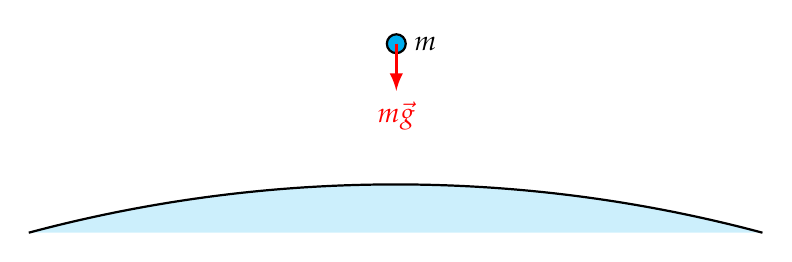
\begin{tikzpicture}[scale=.6]
      \draw[thick,fill=cyan!20] (7.75,0) arc(75:105:30);
      \draw[thick,fill=cyan] (0,4) circle(.2) node[right]{$\;m$};
      \draw[very thick,red,->] (0,4)--(0,3) node[below]{$m\vec g$};
    \end{tikzpicture}
  \end{center}
  \begin{itemize}
  \item Assuming that $\Delta\vec x$ is small, $\vec g$ can be considered to be
    constant
  \item The work done by the gravity ($W_g$) is \emph{positive}, and
    therefore, there is an increase in kinetic energy. The object speeds up.

    \eq{-.2in}{
      W_g=mg\Delta x=\Delta K > 0
    }
  \end{itemize}
\end{frame}



\begin{frame}{Gravitational Potential Energy}
  The work done by gravity can also be expressed in terms of the change in
  height. Using ground as the reference level (i.e.\ $h=0$):
  \begin{center}
    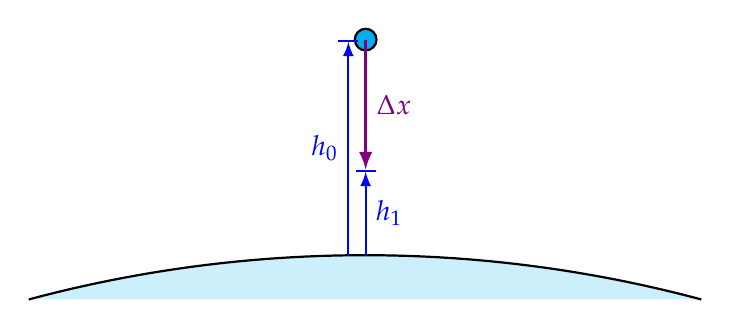
\begin{tikzpicture}[scale=.55,thick]
      \draw[fill=cyan!20] (7.75,0) arc(75:105:30);
      \draw[fill=cyan] (0,6) circle(.25);
      \draw[very thick,violet,->](0,6)--(0,3) node[midway,right]{$\Delta x$};
<<<<<<< HEAD
      \draw[thick,->|,blue](-.4,1)--(-.4,6) node[midway,left]{$h_0$};
      \draw[thick,->|,blue](0,1)--(0,3) node[midway,right]{$h_1$};
    \end{tikzpicture}
  \end{center}

  \vspace{-.3in}{\large
    \begin{align*}
      W_g
      &= mg(h_0-h_1)\\
      &= -mg(h_1-h_0)=-(mgh_1-mgh_0) = -\Delta U_g
    \end{align*}
=======
      \draw[->|,blue](-.4,1)--(-.4,6) node[midway,left]{$h_0$};
      \draw[->|,blue](0,1)--(0,3) node[midway,right]{$h_1$};
    \end{tikzpicture}
  \end{center}

  \eq{-.2in}{
    W_g
    = mg(h_0-h_1)=-mg(h_1-h_0)=-(mgh_1-mgh_0) = -\Delta U_g
>>>>>>> 2022-09-fall
  }
\end{frame}



\begin{frame}{Gravitational Potential Energy}
  Defining the \textbf{gravitational potential energy} $U_g$ as:

  \eq{-.1in}{
    \boxed{U_g=mgh}
  }

  The work done by gravity is related to this potential energy by:
  
  \eq{-.1in}{
    \boxed{
      W_g=-\Delta U_g
    }
  }

  \fcolorbox{black}{yellow!10}{
    \begin{minipage}{.95\textwidth}
      \begin{itemize}
<<<<<<< HEAD
      \item \emph{Positive} work by gravity decreases gravitational potential
        energy, while
      \item \emph{Negative} work by gravity increases gravitational potential
        energy
=======
      \item \emph{Positive} work decreases gravitational potential energy, while
      \item \emph{Negative} work increases gravitational potential energy
>>>>>>> 2022-09-fall
      \item $W_g$ depends on the end points $h_0$ and $h_1$, but not \emph{how}
        it went from $h_0\rightarrow h_1$
      \end{itemize}
    \end{minipage}
  }
\end{frame}



\begin{frame}{Spring Force \& Elastic Potential Energy}
  The spring force $\vec F_s$ is the force that a compressed/stretched spring
  exerts on the object connected to it.  An \emph{ideal} spring obeys Hooke's
  law:
    
  \eq{-.1in}{
    \boxed{\vec F_s=-k\vec x}
  }

  \vspace{-.1in}The spring force acts in the opposite direction to the spring's
  displacement, and is proportional to the amount of compression/stretching.

  \begin{center}
    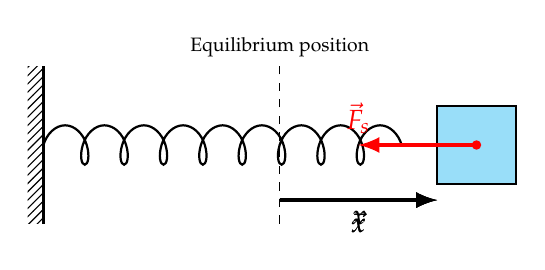
\begin{tikzpicture}
      \draw[thick,fill=cyan!40] (5,.5) rectangle (6,1.5);
      \draw[thick,
        decoration={aspect=.6,segment length=5mm, amplitude=2.5mm, coil},
        decorate] (0,1)--(5,1);
      \fill[pattern=north east lines](-.2,0) rectangle(0,2);
      \draw[thick](0,.0)--(0,2);
      \fill[red] (5.5,1) circle(.06);
      \draw[ultra thick,->,red](5.5,1)--(4,1) node[above]{$\vec F_s$};
      \draw[dashed](3,0)--(3,2) node[above]{\scriptsize Equilibrium position};
<<<<<<< HEAD
<<<<<<< HEAD
      \draw[ultra thick,->](3,.3)--(5,.3) node[midway,below]{$x$};
=======
      \draw[ultra thick,->](3,.3)--(5,.3) node[midway,below]{$\vec x$};
>>>>>>> 0187f47 (A whole bunch of stuff that's changed for Fall of 2022?)
=======
      \draw[ultra thick,->](3,.3)--(5,.3) node[midway,below]{$\vec x$};
>>>>>>> 2022-09-fall
    \end{tikzpicture}
    \hspace{.2in}
    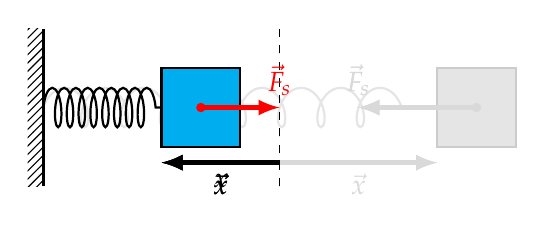
\begin{tikzpicture}
      \draw[thick,gray!40,fill=gray!20] (5,.5) rectangle (6,1.5);
      \draw[thick,gray!20,
        decoration={aspect=.6,segment length=5mm, amplitude=2.5mm, coil},
        decorate] (0,1)--(5,1);
      \fill[pattern=north east lines](-.2,0) rectangle(0,2);
      \draw[thick](0,.0)--(0,2);
      \fill[gray!30] (5.5,1) circle(.06);
<<<<<<< HEAD
<<<<<<< HEAD
      \draw[ultra thick,->,gray!30](5.5,1)--(4,1);
      \draw[dashed](3,0)--(3,2);
      \draw[ultra thick,->,gray!30](3,.3)--(5,.3);
      \draw[thick,fill=cyan!40] (1.5,.5) rectangle (2.5,1.5);
=======
      \draw[ultra thick,->,gray!30](5.5,1)--(4,1) node[above]{$\vec F_s$};
      \draw[dashed](3,0)--(3,2);
=======
      \draw[ultra thick,->,gray!30](5.5,1)--(4,1) node[above]{$\vec F_s$};
      \draw[dashed](3,0)--(3,2);
>>>>>>> 2022-09-fall
      \draw[ultra thick,->,gray!30](3,.3)--(5,.3)node[midway,below]{$\vec x$};
      \draw[thick,fill=cyan] (1.5,.5) rectangle (2.5,1.5);
>>>>>>> 0187f47 (A whole bunch of stuff that's changed for Fall of 2022?)
      \draw[thick,
        decoration={aspect=.3,segment length=1.5mm, amplitude=2.5mm, coil},
        decorate] (0,1)--(1.5,1);
<<<<<<< HEAD
<<<<<<< HEAD
      \draw[ultra thick,->](3,.3)--(1.5,.3) node[midway,below]{$x$};
=======
      \draw[ultra thick,->](3,.3)--(1.5,.3) node[midway,below]{$\vec x$};
>>>>>>> 0187f47 (A whole bunch of stuff that's changed for Fall of 2022?)
=======
      \draw[ultra thick,->](3,.3)--(1.5,.3) node[midway,below]{$\vec x$};
>>>>>>> 2022-09-fall
      \fill[red] (2,1) circle(.06);
      \draw[ultra thick,->,red](2,1)--(3,1) node[above]{$\vec F_s$};
    \end{tikzpicture}
  \end{center}
\end{frame}



\begin{frame}{Elastic Potential Energy}
  \vspace{-.15in}The work done by the spring force $W_e$ as it pushes any
  masses that are connected to a compressed/stretched spring is therefore:

  \eq{-.1in}{
<<<<<<< HEAD
    W_e=\int_{x_0}^{x_1}\vec F_s\cdot\dl\vec x =-k\int_{x_0}^{x_1} x\dl x
    =-\frac12kx^2\Big|^{x_1}_{x_0}=-\Delta U_e
  }

  where $U_e$ is the \textbf{elastic potential energy}, defined as:
=======
    W_s=\int_{x_0}^{x_1}F_s\dl x =-k\int_{x_0}^{x_1} x\dl x
    =-\frac12kx^2\Big|^{x_1}_{x_0}=-\Delta U_s
  }

  where $U_s$ is the  \textbf{elastic potential energy}, defined as:
>>>>>>> 2022-09-fall
  
  \eq{-.1in}{
    \boxed{
      U_s=\frac12kx^2
    }
  }
\end{frame}



\begin{frame}{Elastic Potential Energy}
  The the work done by the spring force can be related to the elastic
  potential energy by:
  
  \eq{-.1in}{
<<<<<<< HEAD
    \boxed{
      W_e=-\Delta U_e
    }
=======
    \boxed{  W_s=-\Delta U_s }
>>>>>>> 2022-09-fall
  }

  \fcolorbox{black}{yellow!10}{
    \begin{minipage}{.95\textwidth}
      \begin{itemize}
      \item \emph{Positive} work by the spring decreases spring potential
        energy, while
      \item \emph{Negative} work by the spring increases spring potential energy
      \item $W_s$ depends on the end points $x_0$ and $x_1$, but not \emph{how}
        it went from $x_0$ to $x_1$
      \end{itemize}
    \end{minipage}
  }
\end{frame}



\begin{frame}{Conservative Forces}
  These forces are called \textbf{conservative forces}
  \begin{itemize}
  \item Gravitational force $\vec F_g$
  \item Spring force $\vec F_s$
  \item Electrostatic force $\vec F_q$
  \item Magnetic force $\vec F_m$
  \item Nuclear forces
  \end{itemize}
  Because they shared these common properties:
  \begin{itemize}
  \item The work done by these forces relate to a change of a potential energy
    \begin{itemize}
    \item Positive work decreases this related potential energy
    \item Negative work increases this related potential energy
    \end{itemize}
  \item The work done by a conservative force is \emph{path independent}
    (depends only on end points)
  \end{itemize}
\end{frame}



\begin{frame}{Conservative Forces}
  By the fundamental theorem of calculus, any conservative forces $\vec F$
  must be the negative gradient of the potential energies:

  \eq{-.1in}{
    \vec F=-\nabla U=
    -\diffp Ux\hat\imath-\diffp Uy\hat\jmath-\diffp Uz\hat k
  }

  In one-dimension:

  \eq{-.1in}{
    \boxed{
      F=-\diff Ux
    }
  }

  The direction of a conservative force \emph{always} decreases the potential
  energy. (Pay attention to the negative sign. Students often forget it.)
\end{frame}



\begin{frame}{Energy Diagrams}
  Plot of potential energy ($U$) vs.\ position ($x$) for a conservative force
  \begin{center}
    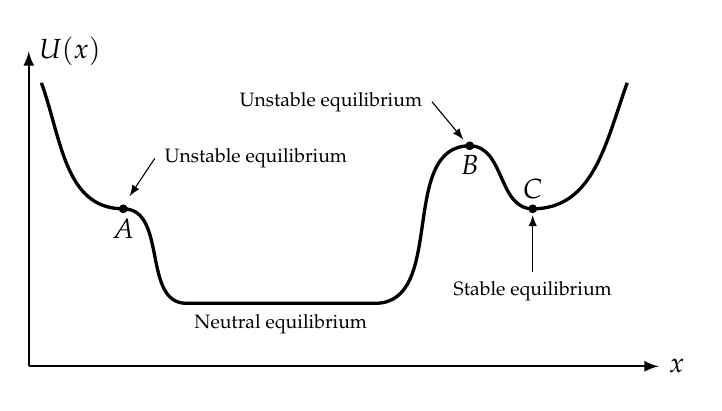
\begin{tikzpicture}[scale=.8]
      \draw[thick,->](0,0)--(10,0) node[right]{$x$};
      \draw[thick,->](0,0)--(0,5) node[right]{$U(x)$};
      \draw[very thick](.2,4.5) to[out=-70,in=180](1.5,2.5)
      to[out=0,in=180](2.5,1)
      --(5.5,1) node[midway,below]{\scriptsize Neutral equilibrium}
      to[out=0,in=180](7,3.5)
      to[out=0,in=180](8,2.5)
      to[out=0,in=250](9.5,4.5);
      \fill(1.5,2.5) circle(.07) node[below]{$A$};
      \fill(7,3.5)   circle(.07) node[below]{$B$};
      \fill(8,2.5)   circle(.07) node[above]{$C$};
      \draw[<-](1.6,2.7)--(2,3.3) node[right]{\scriptsize Unstable equilibrium};
      \draw[<-](6.9,3.6)--(6.4,4.2)node[left]{\scriptsize Unstable equilibrium};
      \draw[<-](8,2.4)--(8,1.5)node[below]{\scriptsize Stable equilibrium};
    \end{tikzpicture}
  \end{center}
\end{frame}

%\begin{frame}{Work and Potential Energy}
%  The expressions for potential energies also come from integrating the work
%  equation, in that work equals to the change in \emph{something}, and we
%  called that potential energy. Therefore:
%
%  \eq{-.2in}{
%    \boxed{
%      W_c=-\Delta U
%    }
%  }
%  \begin{itemize}
%  \item\vspace{-.15in}$\Delta U$ can be positive or negative depending on the
%    direction of the (conservative) force
%  \item Positive work \emph{decreases} the related potential energy
%  \item Negative work \emph{increases} the related potential energy
%  \end{itemize}
%\end{frame}



\begin{frame}{Conservation of Mechanical Energy}
  Positive work done by conservative forces on an object does two things:
  \begin{enumerate}[1.]
  \item Decrease its potential energy, while
  \item Increase its kinetic energy by the same amount
  \end{enumerate}
  Mathematically, this shows that mechanical energy must \emph{always} be
  conserved when there are only conservative forces:

  \eq{-.1in}{
    W_c=-\Delta U = \Delta K \quad\longrightarrow\quad
    \Delta K + \Delta U =0
  }

  That's why those forces are called conservative forces, and they form the
  basis for conservation of energy.
\end{frame}


\section{Non-Conservative Forces}

\begin{frame}{Examples of Non-Conservative Force}
  The majority of forces are \textbf{non-conservative}. The common forces
  discussed in the previous class (and also in Grade 11/12 Physics) are
  generally non-conservative:
  \begin{itemize}
  \item Applied force
  \item Tension force
  \item Normal force
  \item Friction%\footnote{but sometimes it can also do positive work too.}
  \item Drag (fluid resistance)
  \end{itemize}
  The work-energy theorem still applies for non-conservative forces
\end{frame}



\begin{frame}{Work by Non-Conservative Forces}
  The work done by non-conservative forces differs from conservative forces in
  that:
  \begin{itemize}
  \item There is \textbf{no related potential energies}: the work done by a
    non-conservative force transform energy from one form of kinetic energy to
    another
  \item The work is \textbf{path dependent}
  \end{itemize}
\end{frame}



\begin{frame}{Work by Friction, an Illustration}
  Work done by friction---and other non-conservative forces---is illustrated
  below. Two blocks ($m_1$ and $m_2$), stacked vertically, move to the right by
  external force.% $\vec F$ applied to $m_1$.
  \begin{center}
    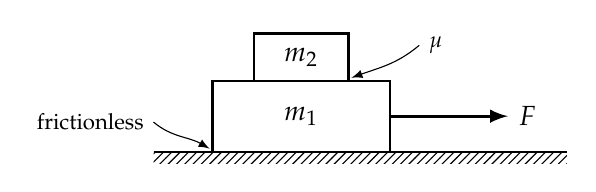
\begin{tikzpicture}[scale=.75]
      \fill[pattern=north east lines] rectangle(7,-.2);
      \draw[thick](0,0)--(7,0);
      \draw[thick](1,0)     rectangle(4,1.2) node[midway]{$m_1$};
      \draw[thick](1.7,1.2) rectangle(3.3,2) node[midway]{$m_2$};
      \draw[->,very thick](4,.6)--(6,.6)     node[right] {$F$};
      \draw[<-](0.95,0.05)to[out=150,in=-40](0,.5)
      node[left]{\footnotesize frictionless};
      \draw[<-](3.35,1.25)to[out=20, in=220](4.5,1.8)
      node[right]{\footnotesize$\mu$};
    \end{tikzpicture}
  \end{center}
  The FBDs of the blocks are shown below. (The forces highlighted in the same
  color are action-reaction pairs.)
  \begin{center}
    \vspace{-.1in}
    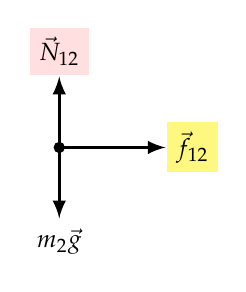
\begin{tikzpicture}[scale=.9]
      \fill circle(.08);
      \begin{scope}[->,very thick]
        \draw(0,0)--(0,-1) node[below]{\small$m_2\vec g$};
        \draw(0,0)--(0, 1) node[above,fill=pink!50]{\small$\vec N_{12}$};
        \draw(0,0)--(1.5,0)node[right,fill=yellow!50]{\small$\vec f_{12}$};
      \end{scope}
    \end{tikzpicture}
    \hspace{.2in}
    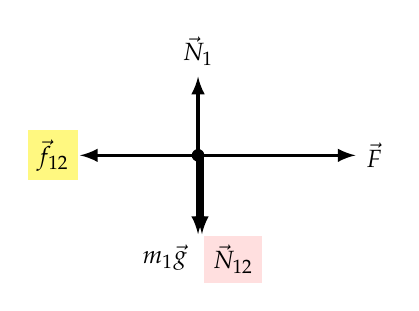
\begin{tikzpicture}
      \fill circle(.08);
      \begin{scope}[->,very thick]
        \draw(0,0)--(0,-1) node[below left]{\small$m_1\vec g$};
        \draw(.05,0)--(.05,-1)
        node[below right,fill=pink!50]{\small$\vec N_{12}$};
        \draw(0,0)--(0, 1) node[above]{\small$\vec N_1$};
        \draw(0,0)--(-1.5,0)node[left,fill=yellow!50]{\small$\vec f_{12}$};
        \draw(0,0)--(2,0)node[right]{\small$\vec F$};
      \end{scope}
    \end{tikzpicture}
  \end{center}
\end{frame}



\begin{frame}{Work by Friction}
  \begin{columns}
    \column{.25\textwidth}
    \centering
    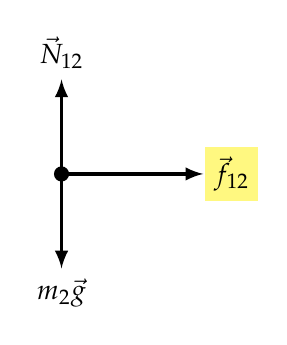
\begin{tikzpicture}[scale=1.2]
      \fill circle(.08);
      \begin{scope}[->,very thick]
        \draw(0,0)--(0,-1) node[below]{$m_2\vec g$};
        \draw(0,0)--(0, 1) node[above]{$\vec N_{12}$};
        \draw(0,0)--(1.5,0)node[right,fill=yellow!50]{$\vec f_{12}$};
      \end{scope}
    \end{tikzpicture}

    \column{.75\textwidth}
    On the top block $m_2$, when it moves to the right
    \begin{itemize}
    \item Friction between the blocks $\vec f_{12}$ is the only force doing work
    \item The work done by $\vec f_{12}$ is positive
    \item Mass $m_2$ gains kinetic energy
    \end{itemize}
  \end{columns}
  \begin{columns}
    \column{.6\textwidth}
    On the bottom block $m_1$, when it moves to the right
    \begin{itemize}
    \item Applied force $\vec F$ does positive work on $m_1$, while
    \item Friction between the blocks $\vec f_{12}$ does negative work
    \item Therefore $\vec f_{12}$ decreases the kinetic energy
    \end{itemize}
    
    \column{.4\textwidth}
    \centering
    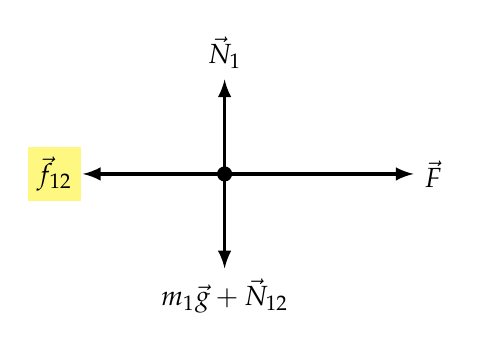
\begin{tikzpicture}[scale=1.2]
      \fill circle(.08);
      \begin{scope}[->,very thick]
        \draw(0,0)--(0,-1) node[below]{$m_1\vec g+\vec N_{12}$};
        \draw(0,0)--(0, 1) node[above]{$\vec N_1$};
        \draw(0,0)--(-1.5,0)node[left,fill=yellow!50]{$\vec f_{12}$};
        \draw(0,0)--(2,0)node[right]{$\vec F$};
      \end{scope}
    \end{tikzpicture}    
  \end{columns}
\end{frame}



\begin{frame}{Work by Friction}
  The work done by friction is
  \begin{itemize}
  \item positive on one object
  \item negative on another
  \end{itemize}
  Therefore, work by non-conservative forces transforms energy from the kinetic
  energy of one object into the kinetic energy of another object.
\end{frame}




\section{Internal Energy}

\begin{frame}{Internal Energy}
  \begin{columns}
    \column{.28\textwidth}
    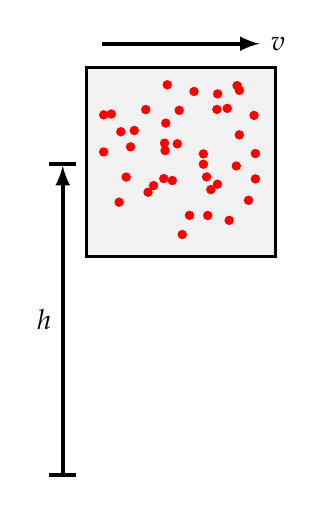
\begin{tikzpicture}
      \draw[very thick,fill=gray!10](-.2,-.2) rectangle(2.2,2.2);
      \draw[line width=.5mm,->](0,2.5)--(2,2.5) node[right]{$v$};
      \draw[line width=.5mm,|<-|](-.5,1)--(-.5,-3) node[midway,left]{$h$};
      \foreach \i in {1,...,40}{
       \fill[red](rand+1,rand+1) circle(.06);
      }
    \end{tikzpicture}

    \column{.72\textwidth}
    Consider a container of gas of mass $M$ moving at speed $v$ at a height $h$
    above Earth. It has a \emph{bulk kinetic energy} of

    \eq{-.1in}{
      K=\dfrac12 Mv^2
    }
    
    and a gravitational potential energy of

    \eq{-.1in}{ U_g=Mgh }

    But the random motion of the air molecules also contribute to additional
    energy, called the \textbf{internal energy} $E_\text{int}$, or
    \textbf{thermal energy}.
  \end{columns}
\end{frame}



\begin{frame}{Internal Energy}
  Internal energy of a system of molecules is the sum of all their kinetic and
  potential energies at the microscopic level:

  \eq{-.1in}{
    \boxed{ E_\text{int}=K_\text{micro} + U_\text{micro} }
  }

  It is a function of the molecules' \textbf{absolute temperature}, measured in
<<<<<<< HEAD
<<<<<<< HEAD
  \emph{kelvin}.
  %For example, 
=======
  \emph{kelvin}. %For example, 
>>>>>>> 0187f47 (A whole bunch of stuff that's changed for Fall of 2022?)
=======
  \emph{kelvin}. %For example, 
>>>>>>> 2022-09-fall
  %\begin{itemize}
  %\item For an ideal gas: $E_\text{int}=\dfrac32NkT$
  %\item For an diatomic gas: $E_\text{int}=\dfrac32NkT$
  %\item Solid: $E_\text{int}=3NkT$
  %\end{itemize}
\end{frame}


\section{Conservation of Energy}

\begin{frame}{Law of Conservation of Energy}
  The \textbf{law of conservation of energy}, which is based on the work-energy
  theorem, states that \emph{the change in the total energy of a system is
    equal to the external work done to it.}

  \eq{-.1in}{
    \boxed{
      \Delta K + \Delta U + \Delta E_\text{int}= W_\text{ext}
    }
  }

  In an isolated system that does not interact with the outside (and therefore
  no external work can be done), conservation of energy reduces to

  \eq{-.1in}{
    \boxed{
      \Delta K + \Delta U + \Delta E_\text{int}= 0
    }
  }

\end{frame}



\begin{frame}{Law of Conservation of Energy}
  In almost all of the problem encountered in AP Physics C, there will be no
  change in the internal energy of the system, and conservation of energy
  reduces to:
  
  \eq{-.1in}{
    \boxed{ \Delta K + \Delta U = W_\text{ext} }\quad\rightarrow\quad
    \boxed{ U_1 + K_1 + W_\text{ext} = U_2 + K_2 }
  }

  External work $W_\text{ext}$ is
  \begin{itemize}
  \item\textbf{Positive} if work is done \text{to} the system
  \item\textbf{Negative} if work is done \text{by} by the system to the
    surrounding
  \end{itemize}
\end{frame}



\begin{frame}{Isolated Systems and the Conservation of Energy}
  An \textbf{isolated system} is a system of objects that does not interact with
  the surrounding. Think of an isolated system as a bunch of objects inside an
  insulated box.
  \begin{center}
    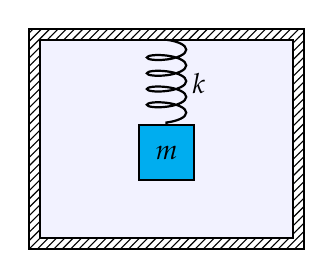
\begin{tikzpicture}[scale=.7]
      \fill[pattern=north east lines] rectangle(5,4);
      \draw[thick] rectangle(5,4);
      \draw[thick,fill=blue!5](.2,.2) rectangle(4.8,3.8);
      \draw[thick,
        decoration={aspect=.3,segment length=2mm, amplitude=2.5mm, coil},
        decorate] (2.5,3.8)--(2.5,2.2) node[midway,right]{$\;\;k$};
      \draw[thick,fill=cyan](2,2.25) rectangle(3,1.25) node[midway]{$m$};
    \end{tikzpicture}
  \end{center}
  Since the system is isolated from the surrounding environment, the
  environment can't do any work on it. Likewise, the energy inside the system
  cannot escape either.
\end{frame}



\begin{frame}{Example: Horizontal Spring-Mass System}
  Assuming that there are no friction, drag or other damping forces present, a
  horizontal spring-mass system is a closed system:
  \begin{center}
    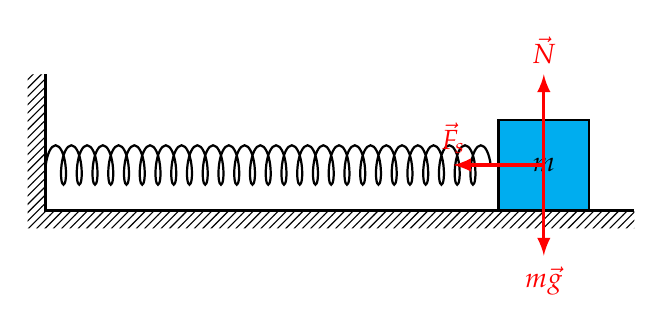
\begin{tikzpicture}[scale=1.15]
      \draw[thick,fill=cyan](5,.5) rectangle(6,1.5) node[midway]{$m$};
      \draw[thick,
        decoration={aspect=.3,segment length=2mm, amplitude=2.5mm, coil},
        decorate] (0,1)--(5,1);
      \fill[pattern=north east lines] (6.5,.5)--(6.5,.3)--(-.2,.3)
      --(-.2,2)--(0,2)--(0,.5)--cycle;
      \draw[very thick] (0,2)--(0,.5)--(6.5,.5);
      \begin{scope}[very thick,->,red]
        \draw (5.5,1)--(5.5,0) node[below]{$m\vec g$};
        \draw (5.5,1)--(5.5,2) node[above]{$\vec N$};
        \draw (5.5,1)--(4.5,1) node[above]{$\vec F_s$};
      \end{scope}
    \end{tikzpicture}
  \end{center}
  The sum of the kinetic energy of the mass ($K$) and the elastic potential
  energy stored in the spring ($U_s$) is constant

  \eq{-.25in}{
    K+U_s=\text{constant}
  }
\end{frame}



\begin{frame}{Example: Gravity}
  Assuming that there are no friction and drag, a free-falling object forms a
  closed system with Earth:
  \begin{center}
    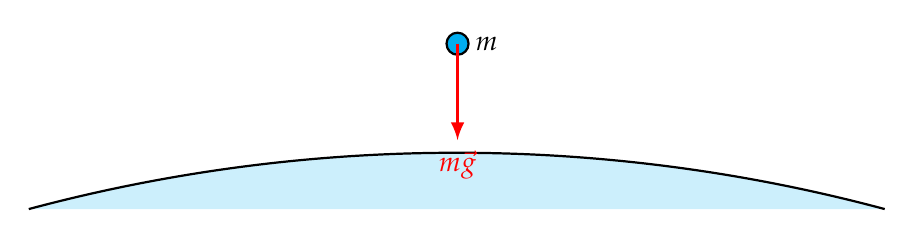
\begin{tikzpicture}[scale=.7]
      \draw[thick,fill=cyan!20] (7.75,0) arc(75:105:30);
      \draw[thick,fill=cyan] (0,3) circle(.2) node[right]{$\;m$};
      \draw[very thick,red,->] (0,3)--(0,1.25) node[below]{$m\vec g$};
    \end{tikzpicture}
  \end{center}
  The sum of the kinetic energy of the mass ($K$) and the gravitational
  potential energy stored between the tow masses ($U_g$) is constant
    
  \eq{-.1in}{
    K+U_g=\text{constant}
  }
\end{frame}



\begin{frame}{Example: Vertical Spring-Mass System}
  \begin{columns}
    \column{.25\textwidth}
    \centering
    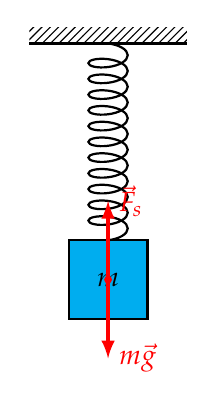
\begin{tikzpicture}
      \draw[thick,fill=cyan](.5,1.5) rectangle(1.5,2.5) node[midway]{$m$};
      \draw[thick,
        decoration={aspect=.4,segment length=2mm, amplitude=2.5mm, coil},
        decorate] (1,5)--(1,2.5); 
      \fill[pattern=north east lines] (0,5) rectangle (2,5.2);
      \draw[very thick](0,5)--(2,5);
      \begin{scope}[very thick,->,red]
        \draw(1,2)--(1,1)node[right]{$m\vec g$};
        \draw(1,2)--(1,3)node[right]{$\vec F_s$};
      \end{scope}
      \fill[red](1,2) circle(.05);      
    \end{tikzpicture}

    \column{.75\textwidth}
    Assuming that there are no friction, drag or other damping forces in the
    spring, the vertical spring-mass system (consists of the mass, the spring
    and Earth) is a closed system.

    \eq{-.1in}{
      K + U_g + U_s=\text{constant}
    }
    
    The sum of the kinetic energy of the mass ($K$), the gravitational
    potential energy stored between the mass and Earth ($U_g$), and the elastic
    potential energy stored in the spring ($U_s$) is constant.
  \end{columns}
\end{frame}



\begin{frame}{Simple Pendulum System}
  \begin{columns}
    \column{.7\textwidth}
    Assuming that there are no friction, drag or other damping forces in the
    spring, the simple pendulum system (consists of the mass and Earth) is a
    closed system.
    \begin{itemize}
    \item Gravity ($m\vec g$), which is conservative, is the only force that
      does work
    \item Tension ($\vec T$), which is non-conservative, does not do work on the
      pendulum because it is always perpendicular to the motion of the pendulum
      bob
    \end{itemize}
    The sum of the kinetic energy of the mass ($K$), the gravitational
    potential energy stored between the mass and Earth ($U_g$) is constant:

    \eq{-.2in}{
      K + U_g =\text{constant}
    }
    
    \column{.3\textwidth}
    \centering
    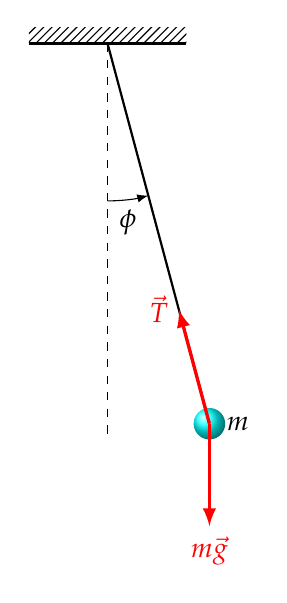
\begin{tikzpicture}
      \fill[pattern=north east lines] (-1,0) rectangle (1,0.2);
      \draw[thick](-1,0)--(1,0);
      \begin{scope}[rotate=15]
        \draw[thick](0,0)--(0,-5);
        \shade[ball color=cyan] (0,-5) circle(.2) node[right]{$\;m$};
        \begin{scope}[red,very thick,->]
          \draw(0,-5)--(0,-3.5) node[left]{$\vec T$};
          \draw[rotate around={-15:(0,-5)}](0,-5)--(0,-6.3)
          node[below]{$m\vec g$};
        \end{scope}
      \end{scope}
      \draw[dashed,thin](0,0)--(0,-5);
      \draw[->](0,-2) arc(270:285:2) node[midway,below]{$\phi$};
    \end{tikzpicture}
  \end{columns}
\end{frame}


\begin{frame}{Isolated System with Changing Internal Energy}
  Energy is always conserved as long as your system is defined properly. In
  this case, the system consists of a mass, a spring, Earth and all the air
  molecules inside the box:
  \begin{center}
    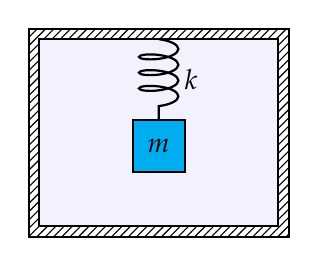
\begin{tikzpicture}[scale=.66]
      \fill[pattern=north east lines] rectangle(5,4);
      \draw[thick] rectangle(5,4);
      \draw[thick,fill=blue!5](.2,.2) rectangle(4.8,3.8);
      \draw[thick,
        decoration={aspect=.3,segment length=2mm, amplitude=2.5mm, coil},
        decorate] (2.5,3.8)--(2.5,2.25) node[midway,right]{$\;\;k$};
      \draw[thick,fill=cyan](2,2.25) rectangle(3,1.25) node[midway]{$m$};
    \end{tikzpicture}
  \end{center}
  The energies of this system include
  \begin{itemize}
  \item Kinetic energy of the mass ($K$)
  \item Gravitational potential energy ($U_g$) between the mass and Earth
  \item Elastic potential energy ($U_s$) stored in the spring
  \item Internal energy ($E_\text{int}$) of the air molecules
  \end{itemize}
\end{frame}



\begin{frame}{Isolated System with Changing Internal Energy}
  As the mass vibrates, friction and drag with air slows it down, converting the
  kinetic energy of the mass into the internal energy of the air. Total energy
  is conserved even as the mass stops moving

  \vspace{.2in}
  \begin{columns}
    \column{.4\textwidth}
    \centering
    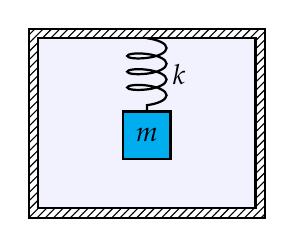
\begin{tikzpicture}[scale=.6]
      \fill[pattern=north east lines] rectangle(5,4);
      \draw[thick] rectangle(5,4);
      \draw[thick,fill=blue!5](.2,.2) rectangle(4.8,3.8);
      \draw[thick,
        decoration={aspect=.3,segment length=2mm, amplitude=2.5mm, coil},
        decorate] (2.5,3.8)--(2.5,2.25) node[midway,right]{$\;\;k$};
      \draw[thick,fill=cyan](2,2.25) rectangle(3,1.25) node[midway]{$m$};
    \end{tikzpicture}

    \column{.6\textwidth}
    \eq{0pt}{
      K + E_\text{int}+U_g+U_s=\text{constant}
    }
  \end{columns}
%
%  \vspace{.2in}Non-conservative forces doing work are \emph{internal} to the
%  system, and therefore energy is still conserved. (Work done by friction
%  transform from the kinetic energy of the mass to the kinetic energy of the
%  air molecules.)
\end{frame}



\begin{frame}{Isolated System vs.\ Open System}
  Accounting for the change in the internal energy of the air molecules is not
  always practical, especially when the air molecules are not confined to a box.
  \begin{center}
    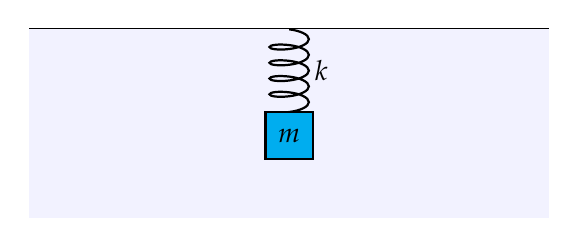
\begin{tikzpicture}[scale=.6]
      \draw[very thick](-3,4)--(8,4);
      \fill[blue!5](-3,0) rectangle(8,4);
      \draw[thick,
        decoration={aspect=.3,segment length=2mm, amplitude=2.5mm, coil},
        decorate] (2.5,4)--(2.5,2.25) node[midway,right]{$\;\;k$};
      \draw[thick,fill=cyan](2,2.25) rectangle(3,1.25) node[midway]{$m$};
    \end{tikzpicture}
  \end{center}
  The solution:
  \begin{itemize}
  \item Take the air molecule out of the \emph{system}
  \item No longer an isolated system
  \item Treat the negative work done by kinetic friction and drag as
    \emph{external work} between initial (1) and final (2) states

    \eq{-.15in}{
      K_1 + U_{g1} + U_{e1} + W_f= K_2 + U_{g2} + U_{e2}
    }
  \end{itemize}
\end{frame}

%\begin{frame}{Conservation of Energy}
%  If \emph{only} conservative forces are doing work, mechanical energy (i.e.\
%  $K+U$) is always conserved:
%
%  \eq{-.2in}{
%    \boxed{K+U =K'+U'}
%  }
%  
%  When external non-conservative forces are also doing work, instead of
%  \emph{trying} to isolate the system, we can instead calculate the work done
%  by them $W_{nc}$ and add it to the total energy of the system
%    
%  \eq{-.2in}{
%    \boxed{K+U+W_{nc}=K'+U'}
%  }
%\end{frame}



\begin{frame}{Example}
  \textbf{Example:} A mass $m$ is dropped from a height of $h$ above the
  equilibrium position of a spring. Set up the equation that determines the
  spring's compression $d$ when the object is instantaneously at rest.
  \begin{center}
    \pic{.35}{spring-example1}
  \end{center}
\end{frame}


%\begin{frame}{Example}
%  \textbf{Example 3:} A mass $m$ is pulled a distance $d$ up an incline (angle
%  of elevation $\theta$) at constant speed using a rope that is parallel to
%  the incline. The coefficient of friction is $\mu_k$.
%  \begin{enumerate}[(a)]
%  \item What is the magnitude of the tension force in the rope?
%  \item What is the magnitude of the normal force?
%  \item What is the work done by the normal force?
%  \item What is the work done by friction?
%  \item What is the work done by the tension force?
%  \item What is the net work?
%  \item What is the change in total mechanical energy?
%  \item Show that $\Delta E_{mech}=W_{nc}$.
%  \end{enumerate}
%\end{frame}



\section{Power \& Efficiency}

\begin{frame}{Power}
  \textbf{Power} is the \emph{rate} at which work is done, i.e.\ the rate at
  which energy is being transformed:

  \eq{-.1in}{
    \boxed{P(t) = \diff Wt}\quad\quad
    \boxed{\overline P = \frac W{\Delta t}}
  }
  \begin{center}
    \begin{tabular}{l|c|c}
      \rowcolor{pink}
      \textbf{Quantity}  & \textbf{Symbol} & \textbf{SI Unit} \\ \hline
      Instantaneous and average power & $P$, $\overline P$ & \si\watt \\
      Work done          & $W$ & \si\joule \\
      Time interval      & $\Delta t$ & \si\second
    \end{tabular}
  \end{center}
  In engineering, power is often more critical than the actual amount of work
  done.
\end{frame}



\begin{frame}{Power}
  If a constant force is used to push an object at a constant velocity, the
  power produced by the force is:
  
  \eq{-.1in}{
    P=\diff Wt=\frac{\vec F\cdot\dl\vec x}{\dl t}
    =\vec F\cdot\diff{\vec x}t
    \quad\rightarrow\quad
    \boxed{P=\vec F\cdot\vec v}
  }
  
  Application: aerodynamics
  \begin{itemize}
  \item When an object moves through air, the applied force must overcome air
    resistance (drag force), which is proportional with $v^2$
    \item Therefore ``aerodynamic power'' must scale with $v^3$ (i.e.\ doubling
      your speed requires $2^3=8$ times more power)
    \item Important when aerodynamic forces dominate
  \end{itemize}
\end{frame}



\begin{frame}{Efficiency}
  \textbf{Efficiency} is the ratio of useful energy or work output to the total
  energy or work input

  \eq{-.1in}{
    \boxed{ \eta = \frac{E_o}{E_i}\times\SI{100}\percent }\quad
    \boxed{ \eta = \frac{W_o}{W_i}\times\SI{100}\percent }
  }
  \begin{center}
    \begin{tabular}{l|c|c}
      \rowcolor{pink}
      \textbf{Quantity} & \textbf{Symbol} & \textbf{SI Unit} \\ \hline
      Useful output energy & $E_o$  & \si\joule \\
      Input energy         & $E_i$  & \si\joule \\
      Useful output work   & $W_o$  & \si\joule \\
      Input work           & $W_i$  & \si\joule \\
      Efficiency           & $\eta$ & no units
    \end{tabular}
  \end{center}
  Efficiency is always $0\leq\eta<\SI{100}\percent$
\end{frame}
\end{document}
